\documentclass[a4paper, twoside, openright, 11pt, oldfontcommands]{memoir}
\usepackage[T1]{fontenc}
\usepackage{microtype}
\usepackage{algorithm}
\usepackage{algpseudocode}
\OnehalfSpacing
\usepackage{cite}
\usepackage{amsmath}
\usepackage{mathtools}
\usepackage{amssymb}
\usepackage{subcaption}
\usepackage{fixltx2e}
\usepackage{hyperref}
\usepackage{stmaryrd}
\hypersetup{
    colorlinks,
    citecolor=black,
    filecolor=black,
    linkcolor=black,
    urlcolor=black
}
\usepackage[authoryear,square]{natbib}
\usepackage{bibentry}
\renewcommand{\cite}{\citep}
\usepackage{tikz}
\usetikzlibrary{arrows.meta,automata,shapes.multipart,positioning}

\let\proof\relax
\let\endproof\relax
\usepackage{amsthm}
\usepackage{xspace}

\algnewcommand{\IIf}[1]{\State\algorithmicif\ #1\ \algorithmicthen}
\algnewcommand{\EndIIf}{}
\algnewcommand{\IfElse}[3]{\algorithmicif\ #1\ \algorithmicthen\ #2\ \algorithmicelse\ #3}
\algnewcommand{\EndIfElse}{}
\algnewcommand{\Break}{\State\textbf{break}}
\MakeRobust{\Call}
\newcommand{\True}{\texttt{true}}
\newcommand{\False}{\texttt{false}}
\newcommand{\II}{\mathcal{I}}
\newcommand{\textoverline}[1]{$\overline{\mbox{#1}}$}

%%% Formatting setup
% 11pt Palatino (URW Palladio) for text
\renewcommand{\rmdefault}{ppl}
% Optima (URW Classico) for headings
%\renewcommand{\sfdefault}{uop}

% Use Courier which has a bold series
\renewcommand{\ttdefault}{pcr}

% Make our pretty chapter headings
% Copied from DaveC via Adam
\usepackage[bf,sf]{titlesec}
\newcommand{\chapformat}[1]{\parbox[c]{0.8\textwidth}{\Huge #1}}
\titleformat{\chapter}[hang]
    {\sffamily\bfseries}
    {\parbox[c]{0.2\textwidth}{\rmfamily\fontsize{72}{72}
     \selectfont\thechapter\hspace{10pt}\rule[-12pt]{2pt}{72pt}}}
    {0pt}
    {\chapformat}

\title{Addressing State Explosion in Reactive Synthesis}

\author{Alexander Legg \\
    \\
    Supervised by \\
Leonid Ryzhyk, Nina Narodytska, and Gernot Heiser}

\begin{document}

\maketitle

\setcounter{secnumdepth}{3}
\setcounter{tocdepth}{3}
\tableofcontents

\newpage

\begin{abstract}

Software controllers of reactive systems are ubiquitous in situations where incorrectness has a high cost. In order to place trust in the software, strong guarantees of its functional correctness are required. Reactive synthesis can be used to automatically construct software to a specification and ensure correctness. The drawback is that synthesis is computationally hard meaning that many specifications are infeasible to synthesise.

Synthesis is hard because reactive systems have many possible states that the synthesis procedure must consider. A standard way to mitigate this complexity is to symbolically represent sets of states with data structures such as binary decision diagrams (BDDs). The usual approach to synthesis is to construct the set of all states that are safe for the controller. In some specifications this set has no compact representation as a BDD and so it is slow or impossible to synthesise a controller in this way.

In this thesis I propose a synthesis algorithm that constructs an approximation of the set of safe states that is sufficient to show correctness of the controller. The algorithm enables synthesis of specifications that were previously infeasible.

\end{abstract}

\newpage

\renewcommand{\abstractname}{Acknowledgements}
\begin{abstract}
Acknowledge some people
\end{abstract}

\newpage

\renewcommand{\abstractname}{Publications}
\begin{abstract}
List publications
\end{abstract}

\chapter{Introduction}

We rely on software systems to perform important tasks for us on a daily basis. Unfortunately we also frequently experience the frustration of an incorrect software system. However, as these systems become more ingrained into our lives the cost of incorrectness can be far greater than mere frustration.

In 1996 the European Space Agency lost their Ariane 5 rocket forty seconds after launch to an incorrect conversion from floating point to integer~\cite{Dowson97}. The cost of the failure was \$370 million in USD. More recently, Toyota has been forced to recall a large number of vehicles due to a failure in the software controlling the brakes~\cite{Parrish13}. The failures led to loss of life~\cite{CBS10}.

As the desire for software and the consequences of incorrectness has grown, the need for a systematic methodology for producing correct software has become apparent. One solution has been to develop strict engineering practices, including rigorous testing, to reduce the chance of errors. Another solution is to produce a proof of correctness of the software, either with or without the aid of a mechanised proof assistant. Model checking can also be used in some cases to automate the correctness proof.

A step further is to have our software automatically constructed for us, a technique first formally considered by Alonzo Church in the middle of the last century~\cite{Church62}. Software synthesis shifts the role of the developer from writing code to writing formal specifications. This completely eradicates the human error factor from the low level construction of software and allows developers to focus on high level system design. In all other approaches to software correctness the software must first be constructed; a process involving considerable time and effort.

Unfortunately, automatic software synthesis involves nontrivial computation. In broad strokes, the synthesis algorithm must determine how the state of the system is affected by the software and its environment and then select actions for the software such that no matter the actions of the environment the system adheres to the specification. In practice, on certain system specifications the process can lead to significant \emph{state explosion} that renders synthesis infeasible.

The state of the art in synthesis contains several methodologies that act as countermeasures to state explosion. However, no single approach is suited to all classes of specifications nor are all specifications currently feasible. In this thesis I propose a methodology for resisting state explosion on a set of synthesis specifications that are problematic for other approaches.

\section{Synthesis}

This thesis is concerned with synthesis of reactive systems. In a reactive system a controller interacts \emph{continuously} with its environment by responding to inputs with the appropriate outputs. For example, a device driver is a reactive system in which the driver interacts with an operating system and a hardware device. Synthesising reactive systems like drivers is different to synthesising regular programs or functions since the correctness of a controller depends on how the system behaves over time instead of a single output corresponding to a single input. As a result, the reactive synthesis problem is staged as a game between the controller and its environment. For a detailed formalisation see Chapter~\ref{ch:background}.

This thesis is concerned with synthesis of controllers for safety games in which the winning condition for the controller is defined by ensuring that the game remains within a set of safe states. The game is zero sum, the environment wins if a state outside the safe set is reached. We say that we have \emph{solved} a game if we can construct a winning strategy for one of the players. The usual approach to solving safety games is to iteratively construct a set of winning states that are known to be safe regardless of the actions of the environment. A winning strategy for the controller can be constructed by choosing actions that have successor states within the winning region.

Explicit enumeration of the states in the winning region is infeasible even on small specifications so the set of states is usually represented symbolically. This is done by specifying the game with states as valuations of a set of boolean variables and using boolean algebra to symbolically define sets of states. Traditionally binary decision diagrams (BDDs) are used to represent boolean functions because they provide compact representations in most cases and there are efficient algorithms for operating on formulas in BDD form. The disadvantage of this approach is that in the worst case the representation occupies space that is exponential in the number of variables in the formula. A BDD is a canonical representation of a formula so it may be the case that a compact BDD representing the winning region for a particular specification does not exist.

Other approaches rely on satisfiability solvers to efficiently perform the operations required by synthesis on sets of states. The satisfiability problem (SAT) is the question of whether a value can be assigned to all variables in a formula such that the formula evaluates to true. Modern SAT solvers provide efficient implementations of backtracking search with computational learning that operate on boolean formulas in clausal normal form (CNF). The advantage of a SAT based approach is that CNF is not canonical so in cases when a BDD cannot compactly represent a set of states it may be possible to do so in CNF.

The disadvantage of SAT based approaches is that solvers only determine whether a satisfying assignment to variables \emph{exists}. This is known as existential quantification. The dual problem, universal quantification, is to determine whether all variable assignments satisfy a formula. Both forms of quantification are required for synthesis in order to decide whether an action exists for one player that satisfies a property for all opponent actions. An example of this kind of computation would be deciding whether the controller can force the game into the winning region regardless of any action the environment chooses. It is possible to perform universal quantification with a SAT solver but it adds considerable complexity, which introduces another bottleneck to the synthesis process.

\section{Approach}

This thesis presents a SAT based approach that computes an approximation of the winning region. By approximating the winning region we hope to avoid the state explosion cost of representing the entire set of winning states. The algorithm is set within a counterexample guided abstraction refinement framework. This is our approach to handling the alternating quantifications of synthesis. Candidate strategies are constructed and refined via counterexamples instead of precisely computing the result of the quantified formula.

In this approach, a SAT solver is used to verify whether a candidate strategy is a winning strategy for a safety game with a fixed number of a game rounds, which we call a bounded game. This approach is similar to bounded model checking where a program is verified by querying a SAT solver for a trace that violates the specification. In our bounded synthesis approach the SAT solver searches for a trace of opponent moves that cause the candidate strategy to lose the bounded game. As with bounded model checking, a counterexample trace informs the algorithm how to refine the candidate strategy.

Discovering a winning strategy for the bounded game does not guarantee that the strategy is winning in the unbounded game. Specifically, if the controller strategy avoids an error state for $k$ rounds this does not guarantee that it can avoid errors for $k+1$ rounds. We address this problem with an extension to the algorithm that iteratively solves bounded games while incrementing the bound. During the execution of the bounded game solver we learn losing states for both players. This computational learning serves a dual purpose by both serving as an optimisation to reduce the search space and also providing the termination condition. By carefully learning states that are losing for the environment we may construct an overapproximation of the environment's winning region. The overapproximation can be used to guarantee that the actual winning region does not contain the initial states and so there cannot be a winning strategy for the environment.


\section{Contribution}

This thesis presents a SAT based counterexample guided approach to controller synthesis of safety specifications. This approach includes a bounded synthesis algorithm, an extension to unbounded synthesis, and a methodology for extracting strategies from the certificate generated by the bounded synthesis algorithm. 

The approach is designed to solve synthesis specifications where the winning region is difficult to represent compactly with existing symbolic techniques. The aim of this work was not to produce a one size fits all approach to safety synthesis but instead to provide a solution suited to some of the problem instances that are difficult to solve for other methods.

The instances that emit winning regions that are difficult to efficiently represent with binary decision diagrams include many real world problems. An example of such a specification is an arbiter that must grant resources from a homogeneous pool in order to fulfil requests from the environment. In this problem the winning region for the environment must exclude all combinations of resource allocations that exceed the number of requests. There is no compact representation of this kind of winning region as a binary decision diagram but in our approach we use overapproximation so that we don't need to find and represent all combinations.

In order to validate the methodology I have implemented the algorithm as an open source tool. In later chapters we present benchmarks that show that the algorithm is promising and although it does not solve as many problem instances as other techniques it performs better on certain classes of problems.


\section{Summary}

\begin{itemize}

    \item \emph{Reactive synthesis} can be used to automatically generate correct-by-construction controllers for software systems. Compared to other approaches to software correctness synthesis does not require the software to first be developed.

    \item Synthesis is formalised as a game between a controller and its environment. In many cases these games can be solved by constructing a symbolic representation of the winning states of the game using a binary decision diagram. However, for some games there is no compact representation of the winning region.

    \item This thesis presents a SAT based counterexample guided approach that targets these cases by constructing an approximation of the winning region that is sufficient to determine the winner of the game.

\end{itemize}


%%%\section{Device Drivers}

%%%Device drivers are the software that allows the operating system to interface
%%%with hardware. The role of the driver is to manipulate the inputs of the device
%%%so that it remains in a error-free state and correctly handles the requests of
%%%the operating system. By way of example consider an ethernet driver. The driver
%%%accepts requests to send and receive data packets from the OS and acts on those
%%%requests by reading from and writing to buffers on the device. It must ensure
%%%that those buffers are maintained in a usable state by correctly updating a
%%%register containing the location of the head of the buffer queue.

%%%According to a study performed in 2011~\cite{Palix11}, drivers account for
%%%approximately 57\% of the lines of code in the Linux kernel and subsequently is
%%%the largest source of bugs. The study also analysed the staging directory of
%%%the kernel, which contains all in-progress drivers, and found it to contain the
%%%highest fault rate (faults per line of code) out of any directory in the
%%%kernel. The results of the study give evidence to the widely held belief that
%%%correct drivers are hard to produce.

%%%Consequences of buggy drivers

%%%This thesis focuses on automatic construction of correct drivers as a solution
%%%to the driver problem. Alternate approaches, of which there are many, will be
%%%discussed in Chapter~\ref{ch:relatedwork}.



\chapter{Formalisation of Software}

Synthesis is a process that demands mathematical formalisation in order to
provide a strong guarantee of the correctness of the resultant software. As
such we require a mathematical language to describe the system we wish to
produce, the environment in which it operates, and the properties we want the
system to adhere to. This chapter will outline that language and the ways we
can reason about what we describe in it.

\section{Reactive Systems}

Devices drivers are an example of a reactive system. A reactive system is a
system that is in a continuous process of responding to input from its
environment. A driver accepts requests from the operating system and state
information from the device, and it responds by sending commands to the device
and reporting to the operating system.

B\"uchi automata~\cite{Buchi62} are a formalisation of reactive systems.
B\"uchi automata are $\omega$-automata, which means they describe finite
systems that accept an infinite stream of input. This is a useful formalism for
synthesis because we want to create finite systems that responds to input
indefinitely.

Like all $\omega$-automata, the language of a B\"uchi automaton is
$\omega$-regular. A regular language over the alphabet $\Sigma$ is

\begin{itemize}
    \item The empty language $\empty$, \emph{or}
    \item A singleton language $\{a\}$ for $a \in \Sigma$, \emph{or}
    \item For two regular languages $A$ and $B$:
    \begin{itemize}
        \item $A \cup B$ the union of those languages, \emph{or}
        \item $A \centerdot B$ the concatenation of those languages, \emph{or}
        \item $A*$ the Kleene operation on that language.
    \end{itemize}
\end{itemize}

An $\omega$-regular language is a regular language with infinitely long words.

\section{Temporal Logic}

Temporal logic takes propositional logic and provides additional semantics for
the concept of time. In order to reason about program executions, which are a
series of discrete steps, the logic must have the expressiveness to talk about
the future.

Linear temporal logic (LTL) allows for statements that refer to a single
execution trace of a system.  Pnueli introduced LTL in 1977~\cite{Pnueli77} to
succinctly describe the outcomes of program execution by referring to global
invariants and eventualities. The syntax is:

\begin{itemize}
    \item $\phi$ is a propositional formula referring to the current state,
    \item $X\phi$ - $\phi$ is true in the next state of the execution,
    \item $F\phi$ - Eventually (finally) $\phi$ will be true, and
    \item $G\phi$ - $\phi$ is always (globally) true.
\end{itemize}

The semantics of this logic is formally defined with respect to 

In 1981 Clarke introduced computation tree logic (CTL)~\cite{Clarke81}, which
has the expressiveness to reason about multiple execution paths of a program.
The syntax of CTL is as follows:

\begin{itemize}
    \item $A\phi$ - $\phi$ is true on all paths
    \item $E\phi$ - there exists a path on which $p$ is true
\end{itemize}

\section{Reactive Synthesis}

\subsection{Synthesis as a Game}

\subsection{GR(1) Games}

\section{Binary Decision Diagrams}

\section{Abstraction}

\section{SAT}

\section{Interpolation}


\chapter{Related Work}
\label{ch:relatedwork}

\chapter{Bounded Synthesis}

\section{Abstract Game Trees}

\section{Algorithm}

\section{Computational Learning}

\section{Optimisation: Strategy Shortening}


\chapter{Strategy Extraction}
\label{ch:strategy}

\newcommand{\strategyext}[0]{\textsc{strategyGen}\xspace}
\newcommand{\genstrategy}{\textsc{strategyGen}}
\newcommand{\strategy}[0]{\textsc{strategy}\xspace}
\newcommand{\partition}[0]{\textsc{partition}\xspace}
\newcommand{\nextf}[0]{\textsc{next}\xspace}
\newcommand{\ogametree}[0]{\mbox{\sc OppGT}}
\newcommand{\eagametree}[0]{\mbox{\sc AbsGT}'}
\newcommand{\pgametree}[0]{\mbox{\sc Cand}}
\newcommand{\apgametree}[0]{\mbox{\sc AbsSolvedGT}}
\newcommand{\opgametree}[0]{\mbox{\sc Spoiling}}

\renewcommand{\ss}[0]{\mathbf{s}}
\newcommand{\cc}[0]{\mathbf{c}}
\newcommand{\uu}[0]{\mathbf{u}}

\newtheorem{theorem}{Theorem}
\newtheorem{example}{Example}
\newtheorem{proposition}{Proposition}

In the previous chapter I introduced an algorithm for solving realisability for bounded safety games. In most applications of synthesis it is desirable to construct a controller strategy rather than merely prove its existence. In this chapter I will introduce a strategy extraction procedure that complements the bounded reachability algorithm. This process takes abstract game trees generated during reachability analysis and, using Craig interpolation, extracts mappings of states to player actions. By using interpolation this step can be done efficiently.

The problem solved in this chapter is related to the extraction of a Skolem function for a QBF. Recall from Chapter~\ref{ch:background} that a Skolem function $f$ provides a mapping from a prefix of universal variables $\hat{y}_0, \hat{y_1}, ..., \hat{y_i}$ to existential variables $\hat{x}$ such that when substituting $\hat{x}$ for $f(\hat{y}_0, \hat{y_1}, ..., \hat{y_i})$ the QBF is equisatisfiable. A Skolem function for a bounded realisability QBF gives a mapping from a prefix of past environment actions to a controller action, i.e. a strategy for that game round. A strategy for the entire game consists of a Skolem function for every round. In this chapter, we construct a strategy by replacing the prefix of previous environment actions with a game state and current environment action pair. This allows us to solve a simpler problem than Skolemisation of the entire QBF by once again taking advantage of the structure of the bounded realisability QBF.

\section{Algorithm}

Recall that a safety game is a tuple $(S, \mathcal{U}, \mathcal{C}, \delta, s_0)$ where $S$ is a set of states, $\mathcal{U}$ a set of environment action variables, $\mathcal{C}$ a set of controller action variables, $\delta$ defines a transition relation, and $s_0$ is an initial state. A winning strategy for controller is a function $\pi^c : 2^{\mathcal{S}} \times 2^{\mathcal{U}} \to 2^{\mathcal{C}}$. A controller strategy is then a mapping from state environment-action pairs to controller actions.

In this chapter we will assume that the safety game is winning for the controller. However, the technique is also easily applied to the environment to extract a spoiling strategy. In computing realisability of a safety game the algorithm constructs a \emph{certificate tree}, which is an abstract game tree $T$ such that for a set of states $s$ and game bound $\kappa$, $s \land \textsc{\textoverline{treeFormula}}(\kappa, \textsc{extend}(T))$ is false. In other words it is a game abstraction for which the environment has no candidate strategy.

We use the certificate tree computed by the game solver as a starting point for strategy generation.  We know that the controller can win the game in $\kappa$ rounds by picking actions from the tree; however we do not yet know which action to choose in which situation.


\subsection{Example}

Figure~\ref{fig:stratExample} introduces the running example for this chapter. It shows a state machine for a game $(\mathcal{S}, \mathcal{U}, \mathcal{C}, \delta, s_0)$ that describes the operation of a simpled clocked flip-flop. For the example we model the clock as part of the game state and assume that it oscillates in every game round. So $\mathcal{S} = \{ c, q, e \}$ is the state space of the game and contains the clock, the previous value of the flip-flop, and an error bit respectively. The environment has a single data bit variable: $\mathcal{U} = \{ d \}$ and the controller has the next value of the flip-flop: $\mathcal{C} = \{ q_n \}$. The diagram shows $\delta$ as a deterministic finite state automaton with edges labelled by a tuple $(d, q_n)$. We use $*$ as a wildcard value to simplify the presentation. The circuit described by the specification allows the environment to save a data bit $d$ into the flip-flop when the clock has a falling edge ($c$ transitions from $1$ to $0$). The controller must correctly set $q_n$ so that $q$ always contains the correct data. The initial state, $s_0$, is $c = 0 \land q = 0 \land e = 0$ and the error set is $e = 1$.

\tikzset{
    pil/.style={
        -{Latex[length=3mm]},
        thick
    },
    snode/.style={
        align=center,
        circle,
        draw,
        thick
    }
}

\begin{figure}
    \centering
    \begin{tikzpicture}
        \node [snode]
            (s1){$c = 0$ \\ $q = 0$ \\ $e = 0$};
        \node [draw=none,left=of s1] (i){};
        \node [snode,below=1.5cm of s1]
            (s0){$c = 1$ \\ $q = *$ \\ $e = 0$};
        \node [snode,right=2.5cm of s0]
            (s3){$c = 0$ \\ $q = 1$ \\ $e = 0$};
        \node [snode,accepting,right=2.5cm of s1]
            (err){$c = *$ \\ $q = *$ \\ $e = 1$};

        \draw [pil] (i) edge (s1);

        \draw [pil] (s0) edge [bend left] node [left] {$(0, 0)$} (s1);
        \draw [pil] (s1) edge [bend left] node [left] {$(*, 0)$} (s0);

        \draw [pil] (s0) edge [bend left] node [below] {$(1, 1)$} (s3);
        \draw [pil] (s3) edge [bend left] node [below] {$(*, 1)$} (s0);

        \draw [pil] (s1) edge node [above] {$(*, 1)$} (err);
        \draw [pil] (s3) edge node [right] {$(*, 0)$} (err);
        \draw [pil] (s0) edge node [above left=0mm and -3mm] {$(*, \lnot d)$} (err);
%%%        \draw [pil] (s1) edge node [below right] {$(*, 0)$} (err);
    \end{tikzpicture}
    \caption{Transition relation of the running example}
    \label{fig:stratExample}
\end{figure}

The strategy generation algorithm takes an initial set $s_0$ and its certificate tree $T$, computed by the game solver, and generates a winning controller strategy starting from $s_0$. We will use $\mathcal{X}$ to denote the union of state and environment action variables $\mathcal{S} \cup \mathcal{U}$. The generated strategy must define a controller action $c \in 2^{\mathcal{C}}$ to every $x \in 2^{\mathcal{X}}$. The algorithm first constructs a set $x$ from $s_0$, which it then partitions into subsets $x_i$, one for each outgoing branch of $T$ (Figure~\ref{fig:partition}), such that the controller can win from $x_i$ by picking action $c_i$ along the $i$th branch of the tree. This partitioning defines the local winning strategy in the root node of $T$.  Next, for each partition $x_i$, the algorithm computes the set of $c_i$-successor states of $x_i$, obtaining the set $x_i'$ of state-action pairs winning in the child subtree $T_i'$ of $T_i$ (Figure~\ref{fig:partition}).  The algorithm is then invoked recursively for each subtree $T_i'$.

\begin{figure}[b]
    \centering
    \captionsetup[subfigure]{width=\textwidth,justification=raggedleft}
    \hspace*{\fill}%
    \begin{subfigure}[t]{.4\textwidth}
        \centering
        \begin{minipage}[t][3cm][t]{\textwidth}
        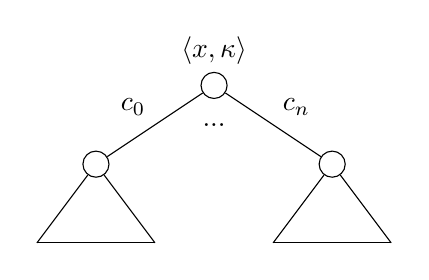
\begin{tikzpicture}[level distance = 10mm,baseline]
            \node [circle,draw] (root){}
                child {node [circle,draw] (left0){}
                    child {node (left1){}
                        edge from parent [draw=none]
                    }
                    child {node (left2){}
                        edge from parent [draw=none]
                    }
                    edge from parent node [above left] {$c_0$}
                }
                child {node [circle] {}
                    edge from parent [draw=none] node [] {$...$}
                }
                child {node [circle,draw] (right0){}
                    child {node (right1){}
                        edge from parent [draw=none]
                    }
                    child {node (right2){}
                        edge from parent [draw=none]
                    }
                    edge from parent node [above right] {$c_n$}
                }
                node [left=4pt] {}
                node [above=4pt] {$\langle x, \kappa \rangle$};

            \draw (left1.center) -- (left2.center);
            \draw (left0) -- (left1.center);
            \draw (left0) -- (left2.center);
            \draw (right1.center) -- (right2.center);
            \draw (right0) -- (right1.center);
            \draw (right0) -- (right2.center);
        \end{tikzpicture}
        \end{minipage}
        \caption{Before}
    \end{subfigure}\hfill%
    \begin{subfigure}[t]{.3\textwidth}
        \centering
        \begin{minipage}[t][3cm][t]{\textwidth}
        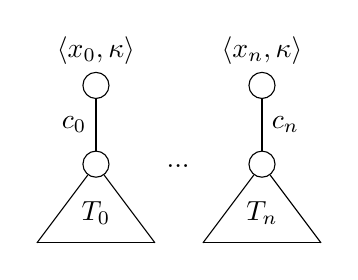
\begin{tikzpicture}[level distance = 10mm,baseline]
            \node [circle,draw] (root){}
                child {node [circle,draw] (left0){}
                    child {node (left1){}
                        edge from parent [draw=none]
                    }
                    child {node (left2){}
                        edge from parent [draw=none]
                    }
                    edge from parent node [left] {$c_0$}
                }
                node [above=4pt] {$\langle x_0, \kappa \rangle$};

            \node [draw=none,below right=25pt and 22pt] {$...$};

            \begin{scope}[xshift=60pt]
            \node [circle,draw] (root2){}
                child {node [circle,draw] (right0){}
                    child {node (right1){}
                        edge from parent [draw=none]
                    }
                    child {node (right2){}
                        edge from parent [draw=none]
                    }
                    edge from parent node [right] {$c_n$}
                }
                node [left=4pt] {}
                node [above=4pt] {$\langle x_n, \kappa \rangle$};
            \end{scope}

            \node [below=5pt of left0] {$T_0$};
            \node [below=5pt of right0] {$T_n$};
            \draw (left1.center) -- (left2.center);
            \draw (left0) -- (left1.center);
            \draw (left0) -- (left2.center);
            \draw (right1.center) -- (right2.center);
            \draw (right0) -- (right1.center);
            \draw (right0) -- (right2.center);
        \end{tikzpicture}
        \end{minipage}
        \caption{After}
    \end{subfigure}%
    \hspace*{\fill}
    \caption{Partitioning}
    \label{fig:partition}
\end{figure}

Figure~\ref{fig:algex} illustrates operation of the algorithm on the winning abstract game tree returned by the game solver for our running example.  Figure~\ref{fig:algexa} displays $T$, the certificate tree for the game. The algorithm starts at the root of the tree and the initial set $x = (c = 0 \land q = 0 \land e = 0)$.  The game tree defines only one winning action in the root node, hence this action is winning in all states of $I$ and no partitioning is required.  We compute the successor set reachable by playing action $q_n = 0$ in $x$: $x' = \textsc{succ}(x, q_n = 0) = (c = 1 \land e = 0) $.

\tikzset{every node/.style={solid}}
\begin{figure}[b]
    \centering
    \captionsetup[subfigure]{width=\textwidth,justification=centering}
    \begin{subfigure}[t]{.4\textwidth}
        \centering
        \begin{minipage}[t][4cm][t]{\textwidth}
        \centering
        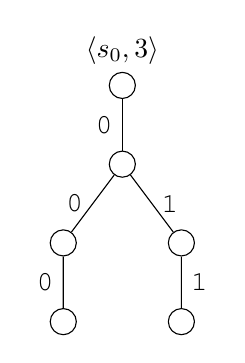
\begin{tikzpicture}[level distance = 10mm,baseline]
            \node [circle,draw] (root){}
                child {node [circle,draw] {}
                    child {node [circle,draw] {}
                        child {node [circle,draw] {}
                            edge from parent node [left] {\texttt{0}}
                        }
                        edge from parent node [left] {\texttt{0}}
                    }
                    child {node [circle,draw] {}
                        child {node [circle,draw] {}
                            edge from parent node [right] {\texttt{1}}
                        }
                        edge from parent node [right] {\texttt{1}}
                    }
                    edge from parent node [left] {\texttt{0}}
                }
                node [above=4pt] {$\langle s_0, 3 \rangle$};
        \end{tikzpicture}
        \end{minipage}
        \caption{$T$}
        \label{fig:algexa}
    \end{subfigure}
    \begin{subfigure}[t]{.4\textwidth}
        \centering
        \begin{minipage}[t][4cm][t]{\textwidth}
        \centering
        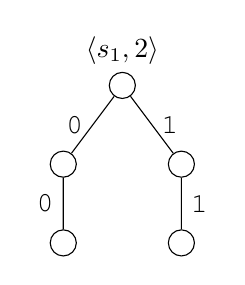
\begin{tikzpicture}[level distance = 10mm,baseline]
            \node [circle,draw] (root){}
                child {node [circle,draw] {}
                    child {node [circle,draw] {}
                        edge from parent node [left] {\texttt{0}}
                    }
                    edge from parent node [left] {\texttt{0}}
                }
                child {node [circle,draw] {}
                    child {node [circle,draw] {}
                        edge from parent node [right] {\texttt{1}}
                    }
                    edge from parent node [right] {\texttt{1}}
                }
                node [above=4pt] {$\langle s_1, 2 \rangle$};
        \end{tikzpicture}
        \end{minipage}
        \caption{$T'$}
        \label{fig:algexb}
    \end{subfigure}
    \begin{subfigure}[t]{.4\textwidth}
        \centering
        \begin{minipage}[t][3cm][t]{\textwidth}
        \centering
        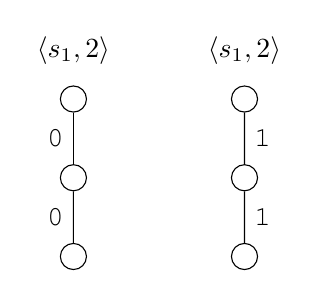
\begin{tikzpicture}[level distance = 10mm,baseline]
            \node [circle,draw] (root1){}
                child {node [circle,draw] {}
                    child {node [circle,draw] {}
                        edge from parent node [left] {\texttt{0}}
                    }
                    edge from parent node [left] {\texttt{0}}
                };
            \node [above=4pt of root1] {$\langle s_1, 2 \rangle$};

            \node [circle,draw,right=2cm] (root2){}
                child {node [circle,draw] {}
                    child {node [circle,draw] {}
                        edge from parent node [right] {\texttt{1}}
                    }
                    edge from parent node [right] {\texttt{1}}
                };
            \node [above=4pt of root2] {$\langle s_1, 2 \rangle$};
        \end{tikzpicture}
        \end{minipage}
        \caption{AGT}
        \label{fig:algexc}
    \end{subfigure}%
    \begin{subfigure}[t]{.4\textwidth}
        \centering
        \begin{minipage}[t][3cm][t]{\textwidth}
        \centering
        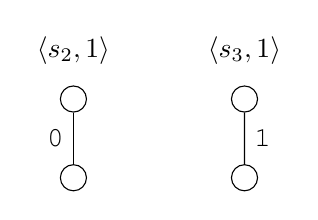
\begin{tikzpicture}[level distance = 10mm,baseline]
            \node [circle,draw] (root1){}
                child {node [circle,draw] {}
                    edge from parent node [left] {\texttt{0}}
                };
            \node [above=4pt of root1] {$\langle s_2, 1 \rangle$};

            \node [circle,draw,right=2cm] (root2){}
                child {node [circle,draw] {}
                    edge from parent node [right] {\texttt{1}}
                };
            \node [above=4pt of root2] {$\langle s_3, 1 \rangle$};
        \end{tikzpicture}
        \end{minipage}
        \caption{$T''$}
        \label{fig:algexd}
    \end{subfigure}
    \caption{Operation of the strategy extraction algorithm on the example}
    \label{fig:algex}
\end{figure}

Next, we descend down the tree and consider subtree $T'$ and its initial set $x'$ (Figure~\ref{fig:algexb}).  We partition $x'$ into subsets $x_0' = (d = 0 \land c = 1 \land e = 0)$ and $x_1' = (d = 1 \land c = 1 \land e = 0)$ that are winning for the left and right subtrees of $T'$ respectively, i.e., from $(c = 1 \land e = 0)$ the controller must play action $q_n = 0$ when the environment plays $d = 0$ and $q_n = 1$ for $d = 1$.  Consider the resulting subtrees $T'_1$ and $T'_2$ with initial sets $x'_1$ and $x'_2$ (Figure~\ref{fig:algexc}).  We have $x''_1 = \textsc{succ}(x'_1, q_n = 0) = (c = 1 \land q = 0 \land e = 0)$, $x''_2 = \textsc{succ}(x'_2, q_n = 1) = (c = 1 \land q = 1 \land e = 0)$.  Finally, we obtain two subtrees $T''_1$ and $T''_2$ with initial sets $x''_1$ and $x''_2$ (Figure~\ref{fig:algexd}).  Both subtrees have one branch; hence corresponding actions $q_n = 0$ and $q_n = 1$ are winning in $x''_1$ and $x''_2$ respectively.

Putting together fragments of the winning strategy computed above, we obtain the following strategy for this example:
\begin{align*}
    \pi(c = 0 \land q = 0 \land e = 0) &= (q_n = 0) \\
    \pi(d = 0 \land c = 1 \land e = 0) &= (q_n = 0) \\
    \pi(d = 1 \land c = 1 \land e = 0) &= (q_n = 1) \\
    \pi(c = 0 \land q = 1 \land e = 0) &= (q_n = 1)
\end{align*}

The above algorithm involves two potentially costly operations: winning set partitioning and successor set computation.  If implemented na\"ively, these operations can lead to unacceptable performance.  The key insight behind our solution is that both operations can be efficiently approximated from the proof of unsatisfiability of the formula $s_0 \land \texttt{treeFormula}(T)$, with the help of interpolation, as described below.  The resulting approximations are sound, i.e., preserve the correctness of the resulting strategy.

\subsection{Local Strategies}

Algorithm~\ref{alg:strat} shows the pseudocode of the strategy generation algorithm.  The algorithm proceeds in two phases: the first phase (\textsc{genLocalStrats}) computes local strategies in nodes of $T$; the second phase (\textsc{compileStrat}) compiles all local strategies into a winning strategy function.

The \textsc{genLocalStrats} function recursively traverses the certificate tree $T$, starting from the root, computing local strategies in each node.  The main operation of the algorithm, called \textsc{partition}, splits $(T,x)$ into $j$ pairs $(T_i, x_i)$, as shown in Figure~\ref{fig:partition}.  Each tree $T_i$ is a copy of a single branch of $T$.  The partitioning is constructed in such a way that the action $c_i$ that labels the root edge of $T_i$ is a winning controller action in $x_i$.

Next we consider each pair $(T_i, x_i)$ (lines~\ref{alg:strat:for}-\ref{alg:strat:endfor}). We descend down the tree and compute the controller strategy in the child subtree $T_i'$ of $T_i$ (right-hand side of Figure~\ref{fig:partition}).  To do so, we first compute the set of $c_i$-successors of $x_i$: More precisely, we compute an overapproximation $x_i' \supseteq succ(x_i, c_i)$, such that $T_i'$ is a certificate tree for $x_i'$.  Such an overapproximation is returned by the \textsc{next} function in line~\ref{alg:strat:next}.  We can now recursively invoke the strategy generation function to compute a winning strategy for the pair $(T_i', x_i')$ (line~\ref{alg:strat:rec}).

\begin{algorithm}
   \caption{Computing a winning strategy}\label{alg:strat}
   \begin{algorithmic}[1]
        \Function{GenStrategy}{$T$, $x$}
            \State $Strat \gets \Call{GenLocalStrats}{T,x}$
            \State \Return{$\Call{CompileStrat}{Strat}$}
        \EndFunction
        \Statex

        \Function{GenLocalStrats}{$T$, $x$}
            \State $[(e_1, n_1),\ldots,(e_j, n_j)] \gets \Call{succ}{T}$
            \State $[(T_1,x_1),\ldots,(T_j, x_j)] \gets \partition(T, x \land \neg E(\mathcal{S}_T))$
            \State $Strat \gets \{(x_i, \Call{action}{e_i}, \Call{height}{T}) \mid i \in[1,..,j]\}$\label{alg:strat:strati}
            \For{$i = 1$ to $j$}\label{alg:strat:for}
                \State $(T_i', x_i') \gets \nextf(T_i, x_i)$\label{alg:strat:next}
                \State $Strat_i \gets \Call{GenLocalStrats}{T_i', x_i'}$\label{alg:strat:rec}
                \State $Strat \gets Strat \cup Strat_i$
            \EndFor\label{alg:strat:endfor}
            \State \Return{$Strat$} \label{alg:strat:return}
        \EndFunction
    \end{algorithmic}
\end{algorithm}

The algorithm returns the set of tuples $(W, c, k)$.  Each tuple represents a fragment of the strategy in some tree node, where $W$ is the winning set in this node, $c$ is the controller action to play in this set, and $k$ is the distance from the node to the bottom of the tree.

\subsection{Partitioning game trees}

The \textsc{partition} function (Algorithm~\ref{alg:strat:partition}) computes a local strategy in the root of an abstract game tree.  It takes a pair $(T, x)$, such that $T$ is a certificate tree for set $x$ and partitions $x$ into subsets $x_i$ such that the controller can win by choosing action $c_i$ in $x_i$.

\begin{algorithm}[t]
   \caption{Partitioning winning states}\label{alg:strat:partition}
   \begin{algorithmic}[1]
        \Function{$\partition$}{$T$, $x$}
        \State $\hat{x} \gets x$
        \State $\hat{T} \gets T$
        \For{$i = 1$ to $j$}
        \State $(T_i, \tilde{T}) \gets \Call{split}{\hat{T}}$\label{alg:partition:split}
            \State $A \gets \hat{x} \land \Call{treeFormula}{\tilde{T}} $ \label{alg:strat:partition:Bi}
            \State $B \gets \Call{treeFormula}{T_i} $ \label{alg:strat:partition:Ai}
            \State $\mathcal{I}(s_v) \gets \Call{interpolate}{A, B}$\label{alg:partition:I}
            \State $x_i \gets \mathcal{I}(s) \land \hat{x}$\label{alg:partition:Ii}
            \State $\hat{x} \gets \hat{x} \land \neg\mathcal{I}(s)$,~~$\hat{T} \gets \tilde{T}$\label{alg:partition:upd}
        \EndFor
        \State \Return{$[(T_1, x_1),\ldots, (T_j, x_j)]$} \label{alg:strat:partition:return}
        \EndFunction
    \end{algorithmic}
\end{algorithm}

At every iteration, the algorithm splits the tree into the leftmost branch $T_i$ and the remaining tree (Figure~\ref{fig:split}).  It then computes the set $x_i$ where the controller wins by following the branch $T_i$ and removes $x_i$ from the initial set $x$.  At the next iteration it considers the leftover tree $\tilde{T}$ and the shrunk initial set $\hat{x}$.

\begin{figure}
    \centering
    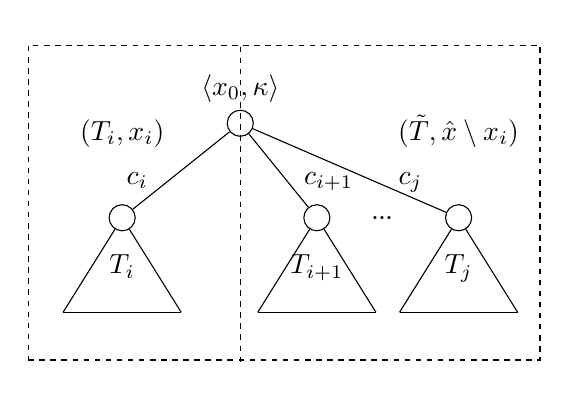
\begin{tikzpicture}[level distance = 12mm,baseline]
        \node [circle,draw] (root){}
            child {node [circle,draw] (left0){}
                child {node (left1){}
                    edge from parent [draw=none]
                }
                child {node (left2){}
                    edge from parent [draw=none]
                }
                edge from parent node [below left=-1mm and 3mm] {$c_i$}
            }
            child {node [circle,draw,right=8mm] (leftb0){}
                child {node (leftb1){}
                    edge from parent [draw=none]
                }
                child {node (leftb2){}
                    edge from parent [draw=none]
                }
                edge from parent node [below right=-1mm and 2mm] {$c_{i+1}$}
            }
            child {node [circle,draw,right=11mm] (leftc0){}
                child {node (leftc1){}
                    edge from parent [draw=none]
                }
                child {node (leftc2){}
                    edge from parent [draw=none]
                }
                edge from parent node [below right=-1mm and 5mm] {$c_{j}$}
            }
            node [above=4pt] {$\langle x_0, \kappa \rangle$};


        \node [draw,
            dash pattern=on 2pt off 2pt,
            minimum width=6.5cm,
            minimum height=4cm,
            below right=-10mm and -27mm
            ] {};
        \node [above=8mm of root] (startline) {};
        \node [below=29mm of root] (endline) {};
        \draw [dash pattern=on 2pt off 2pt] (startline) -- (endline);

        \node [below=5pt of left0] {$T_i$};
        \node [below=5pt of leftb0] {$T_{i+1}$};
        \node [below=5pt of leftc0] {$T_j$};
        \draw (left1.center) -- (left2.center);
        \draw (left0) -- (left1.center);
        \draw (left0) -- (left2.center);
        \draw (leftb1.center) -- (leftb2.center);
        \draw (leftb0) -- (leftb1.center);
        \draw (leftb0) -- (leftb2.center);
        \draw (leftc1.center) -- (leftc2.center);
        \draw (leftc0) -- (leftc1.center);
        \draw (leftc0) -- (leftc2.center);
        \node [right=4mm of leftb0] {...};
        \node [above=6mm of left0] {$(T_i, x_i)$};
        \node [above=6mm of leftc0] {$(\tilde{T}, \hat{x} \setminus x_i)$};
    \end{tikzpicture}
    \caption{Splitting of $T$ in the \textsc{Partition} function.\label{fig:split}}
\end{figure}

The algorithm maintains the invariant that $\hat{T}$ is a certificate tree for $\hat{x}$ and hence $\lnot \hat{x} \land \textsc{treeFormula}(\hat{T})$ is unsatisfiable.  We decompose this formula into two conjuncts $A \land B$ such that $A$ and $B$ only share state and action variables $\mathcal{S}_T \cup \mathcal{U}_T$ in the root node of $T$ and that the interpolant $\mathcal{I}$ of $A$ and $B$ consists of states and environment actions for which the controller can win by following the $T_i$ subtree.  Hence $\mathcal{I}\land \hat{x}$ gives us the desired set $x_i$.  

Informally, $A$ is a partial expansion of the game formula induced by $\tilde{T}$.  It is satisfiable iff there exists a spoiling environment strategy from $\hat{x}$ against abstract game tree $\tilde{T}$.  $B$ is a partial expansion of the game induced by $T_i$.  It is satisfiable iff there exists a spoiling environment strategy against $T_i$.  Both $A$ and $B$ can be satisfiable individually, but their conjunction is unsatisfiable.

The interpolant $\mathcal{I}$ of $A$ and $B$ implies $\neg B$, i.e., for any state and environment action in $\mathcal{x}$, $c_i$ is a winning move.  $\mathcal{I}$ is also implied by $A$, i.e., it contains all states and environment actions in $x$ where the controller cannot win by picking moves from $\tilde{T}$ as a subset.  Equivalently, for any state and action in $x_i \land \neg \mathcal{I}$, the controller \emph{can} win by following $\tilde{T}$, i.e., $\tilde{T}$ is a certificate tree for $x_i \land \neg \mathcal{I}$, and we can apply the decomposition again to $\tilde{T}$ and $x_i \land \neg \mathcal{I}$ at the next iteration.


We prove useful properties of the $\partition$ function. We begin with the proposition that $A$ and $B$ form a conjunctive decomposition of $\hat{x} \land \textsc{treeFormula}(\hat{T})$. 
\begin{proposition}\label{prop:aandb}
    $A\land B = \hat{x} \land \textsc{treeFormula}(\hat{T})$.
\end{proposition}
\begin{proof}
    \begin{align*}
        A \land B &= \hat{x} \land \textsc{treeFormula}(\tilde{T}) \land \textsc{treeFormula}(T_i) \\
                  &= \hat{x} \land \textsc{treeFormula}(\hat{T})\ \text{(by the definition of \textsc{treeFormula})}
    \end{align*}
\end{proof}

\begin{proposition}
    The following invariant is maintained throughout the execution of
    \textsc{partition}: $\hat{T}$ is a certificate tree for $\hat{x}$.
\end{proposition}
\begin{proof}
We prove by induction.  The invariant holds for the initial
assignments of $\hat{T}$ and $\hat{x}$. By Proposition~\ref{prop:aandb} and induction hypothesis, $A\land B = \hat{x} \land \textsc{treeFormula}{\hat{T}}$ is unsatisfiable.  Hence the interpolation operation in line~\ref{alg:partition:I} is well defined.  By the properties of interpolants, $(A \implies \mathcal{I}(\mathcal{X}_T))$, hence $(\neg \mathcal{I}(\mathcal{X}_T) \implies \neg A)$ or equivalently $(\neg\mathcal{I}(\mathcal{X}_T) \implies \neg (\hat{x} \land \textsc{treeFormula}(\tilde{T}))$.

After $\hat{T}$ and $\hat{x}$ are updated in line~\ref{alg:partition:upd}, their new values $\hat{T}'$ and $\hat{x}'$ satisfy the following equalities: \begin{align*}
    \hat{x}' \land \textsc{treeFormula}(\hat{T}') =& \hat{x} \land \textsc{treeFormula}(\tilde{T}) \land \neg\mathcal{I}(\mathcal{X}) \\
=& \neg\mathcal{I}(\mathcal{X}_v) \land \hat{x} \land \textsc{treeFormula}(\tilde{T}) \\
    \implies& \neg (\hat{x} \land \textsc{treeFormula}(\tilde{T})) \land \hat{x} \land \textsc{treeFormula}(\tilde{T}) \\
    =& \bot
\end{align*} and hence the invariant is maintained.
\end{proof}

\begin{proposition}\label{prop:partition}
    Let $T$ be a certificate tree for $I$ and let $I\land O =\bot$.  Then
    $[(T_1,I_1),\ldots,(T_j, I_j)] = \textsc{partition}(T, I)$
    is a local winning strategy in the root of $T$, i.e., the
    following properties hold:
    \begin{enumerate}
        \item Sets $I_1,\ldots,I_j$ comprise a partitioning of
            $I$: $I=\bigvee I_i$ and $\forall i, k. (i\neq k)
            \implies I_i\land I_k=\bot$
        \item $T_i$ is a certificate tree for $I_i$, for all
            $i\in[1,j]$
    \end{enumerate}
\end{proposition}
\begin{proof}
    At every iteration of the algorithm, we partition $\hat{I}$
    into $I_i = \mathcal{I} \land\hat{I}$ and
    $\hat{I} \land \neg\mathcal{I}$; hence different sets $I_i$ do
    not overlap by construction.

    At the final iteration of the algorithm, the tree $\tilde{T}$
    consists of a single root node without outgoing branches.
    Hence, $A = E_{\tilde{T}}(\hat{I}) = \hat{I}(s_v) \land \neg O(s_v) =
    \hat{I}(s_v)$.  Since $(A\implies \mathcal{I}(s_v))$, we get $(\hat{I} \implies \mathcal{I}(s))$
    and therefore $\mathcal{I}(s) \land \hat{I} = \hat{I}$, i.e., all
    states in $\hat{I}$ are included in the final set $I_j$ and hence
    the partitioning completely covers set $I$: $I=\bigvee I_i$.

    We prove the second statement of the proposition.  The set $I_i$ is computed as
    $\mathcal{I}(s) \land \hat{I}$ (line~\ref{alg:partition:Ii}) at the $i$th iteration of the algorithm.
    Thus, $E_{T_i}(I_i) = E_{T_i}(\mathcal{I}(s) \land \hat{I}) = \mathcal{I}(s) \land \hat{I} \land E_{T_i}(\top)$.
    By the properties of interpolants, $\mathcal{I}(s) \land B = \mathcal{I}(s) \land E_{T_i}(\top) = \bot$.
    Hence $E_{T_i}(I_i) = \bot$, i.e., $T_i$ is a certificate tree for $I_i$.
    \qed
\end{proof}

\subsection{Determine an action}

The \textsc{next} function (Algorithm~\ref{alg:next}) takes a set $I$ and its certificate tree $T$, such
that there is exactly one outgoing edge, labelled $a$, from the root node of $T$.
$T$ has a sole child subtree $T'$ with root node $v'$.
The function computes an overapproximation $I'$ of the $a$-successor of $I$,
such that $I'$ is winning for the controller and $T'$ is a certificate tree for $I'$.

\begin{algorithm}[t]
   \caption{Successor set}\label{alg:next}
   \begin{algorithmic}[1]
        \Function{$\nextf$}{$T, I$}
            \State $T' \gets subtree(T, 1)$
            \State $v \gets root(T)$
            \State $[(e,a,v')] \gets edges(v)$
            \State $A \gets I(s_v) \land  \Delta(s_v, c_e, u_e, s_{v'}) \land c_e = a$\label{alg:strat:partition:Ai}
            \State $B \gets E_{T'}(\top)$\label{alg:strat:partition:Bi}
            \State $\mathcal{I}(s_{v'}) \gets Interpolant(A, B)$\label{alg:strat:partition:I}
            \State \Return{$(T', \mathcal{I}(s))$} \label{alg:strat:partition:return}
        \EndFunction
    \end{algorithmic}
\end{algorithm}

Once again, we decompose the unsatisfiable formula $E_T(I)$ into
two conjuncts $A$ and $B$.  $A$ encodes one round of the game
from the set $I$, where the controller plays action $a$.
$B = E_{T'}(\top)$ is a partial $\forall$-expansion of the game induced by $T'$.
$A$ and $B$ only share state variables $s_{v'}$ and their interpolant
gives the approximation we are looking for.

\begin{proposition}\label{prop:next}
    Let $T$ be a certificate tree for $I$ with a single outgoing
    edge, labelled $a$ in its root node, and let $(T',\mathcal{I})
    = \textsc{next}(T,I)$.
    Then:
    \begin{enumerate}
        \item $\mathcal{I}$ is an overapproximation of the
            $a$-successor of $I$, i.e., $\mathcal{I} \supseteq
            succ(I, a)$
        \item $T'$ is a certificate tree for $I'$
    \end{enumerate}
\end{proposition}
\begin{proof}
We rewrite formula~(\ref{eq:succ}) in the symbolic form:
$succ(I, a) = \exists s_v,u_e. I(s_v) \land
\Delta(s_v,c_e,u_e,s_{v'}) \land c_e = a$.  The matrix of
this formula is exactly formula $A$.  Hence $succ(I,a) =
\exists s_v,u_e. A$.  Since $(A\implies
\mathcal{I}(s_{v'}))$, $succ(I,a) \implies \exists s,u.
\mathcal{I}(s_{v'})$.  Since $\mathcal{I}$ is defined over
state variables only, the quantifiers can be removed:
$succ(I,a) \implies \mathcal{I}(s_{v'})$ or, in the
relational form, $\mathcal{I} \supseteq succ(I, a)$.
We prove the second property:
$E_{T'}(\mathcal{I}) = \mathcal{I}(s_{v'}) \land
E_{T'}(\top) = \mathcal{I}(s_{v'}) \land B = \bot$.
    \qed
\end{proof}

\subsection{Compiling the strategy}

Finally, we describe how local strategies computed by
\textsc{genLocalStrats} are combined into a winning strategy for
the game.  This requires some care, as individual partial
strategies can be defined over overlapping sets of states.  We
want the resulting strategy function to be deterministic;
therefore for each partial strategy we only add new states not yet
covered by the computed combined strategy.  Function
\textsc{compileStrats} (Algorithm~\ref{alg:compile}) achieves this by keeping track of all
states $W$ already added to the strategy.  For every new tuple $(I, a,
k)$, it restricts the set $I$ to $\neg W$, which guarantees that no
state can be added to the strategy twice.  Furthermore, by
considering tuples with smaller values of $k$ first, we resolve the
nondeterminism in a way that guarantees progress towards the goal
at every round of the game.

\begin{algorithm}[t]
   \caption{Compiling the  winning strategy}\label{alg:compile}
   \begin{algorithmic}[1]
        \Function{CompileStrat}{$Strat$}
            \State $\pi \gets \bot,~~W \gets \bot$
            \For{$(I, a, k) \in Strat$} \Comment{Sorted by ascending $k$}
                \State $\pi \gets \pi \lor (I \land \neg W \land (c=a))$
                \State $W \gets W \lor I$
            \EndFor
            \State \Return $\pi$
        \EndFunction
    \end{algorithmic}
\end{algorithm}

Let $rank(s), s\in S$, be the smallest $k$ such that there exists
$(I,a,k) \in Strat$, $s \in I$, or $\infty$ if there is no such
$k$.

\begin{proposition}\label{prop:rank}
    Let $\pi=\textsc{compileStrat}(Strat)$. For any pair $(s,a)
    \in \pi$, there exists $(I, a, k) \in Strat$ such that $s\in
    I$ and $k=rank(s)$.
\end{proposition}

%We state the main correctness theorem.  The theorem states that
%the algorithm computes a correct winning strategy for the
%controller.

\begin{theorem}[Correctness of the algorithm]
Let abstract game tree $T$ of height $n$ be a certificate tree for
the set $I$, let $\pi$ be a partial function returned by the
strategy generation algorithm, $\pi=\textsc{genStrategy}(T,I)$,
and let $\pi'$ be an arbitrary extension of $\pi$ to a complete
function.  Then $\pi'$ is a winning controller strategy of length
$n$ from $I$.
\end{theorem}
\begin{proof}
Every state-action pair $(s, a)$ in $\pi$ is generated by the
\textsc{partition} function and, according to
Proposition~\ref{prop:partition}, $a$ is a winning controller move
in $s$. By Proposition~\ref{prop:next}, all possible
$a$-successors of $s$ are either goal states or are covered by
$\pi$.  Hence, by following the strategy $\pi$ from $I$, the
controller is guaranteed to stay within the winning region of the
game until reaching the goal.

Next, we show that ranks of states visited by following the
strategy $\pi$ decrease monotonically and hence the strategy
reaches the goal in at most $n$ steps. According to
Proposition~\ref{prop:rank}, for every pair $(s,a) \in \pi$, there
exists $(I, a, k)\in Strat$, such that $k=rank(s)$.  Therefore,
for any $s'\in succ(s,a)$, such that $s'\not\in O$, there exists
$(I', a', k-1)\in Strat$, $s'\in I'$; hence $rank(s')\leq k-1 < k
= rank(s)$.
\qed
\end{proof}

\section{Related work}

\section{Conclusion}


\chapter{Unbounded Realisability}
\label{ch:unbounded}

\newtheorem*{exmpInt}{Example: Why we use interpolants}

In previous chapters I outlined an algorithm to solve bounded realisability games and an extension that can extract strategies from the result. Bounded realisability can be used to prove the existence of a winning strategy for the environment on the unbounded game by providing a witness. For the controller, the strongest claim that can be made is that the strategy is winning as long as the game does not extend beyond the maximum bound. The work described in this chapter can be used to address this by presenting another extension to the algorithm that solves unbounded realisability games.

The baseline solution to this problem is to set a maximum bound such that all runs in the unbounded game will be considered. The na\"ive approach is to use size of the state space as the bound (${|\mathcal{X}|}$) so that all states may be explored by the algorithm. A more nuanced approach is to use the diameter of the game \cite{biere1999}, which is the smallest number $d$ such that for any state $x$ there is a path of length $\leq d$ to all other reachable states. Computing the diameter, however, is also expensive and solving a game bounded to the size of the diameter may be infeasible.

Instead I present an approach that iteratively solves games of increasing
bound while learning bad states from abstract games using Craig interpolation. We utilise the approximation properties of the interpolant to construct sets of states that underapproximate the total losing set for the controller. By underapproximating we avoid constructing a potentially large representation of this set that could be the cause of infeasibility in a BDD solver. Later in this chapter we will see that a careful construction of approximate sets enables a fixed point that is sufficient to prove the nonexistence of an environment-winning strategy.

%%%\subsection{Extending Bounded Synthesis to Unbounded Games}


%%%During the CEGAR loop of the bounded algorithm, each of the competing solvers
%%%searches for satisfying assignments of labels to abstract game trees. When the
%%%abstract game is unsatisfiable this indicates that the states represented by
%%%nodes in the abstract game tree are losing for the current player. We extract
%%%these states from the game tree using interpolation.

%%%When executing the unbounded solver, lines 19 and 20 become active in the
%%%bounded solver. These lines call the learning procedures when the solver fails
%%%to find a candidate for an abstract game tree. The states symbolically
%%%represented by nodes in the tree are losing for whichever player could not find
%%%a winning candidate and can be extracted from the tree using interpolation.

%%%The states in an abstract game with no controller candidate are
%%%\emph{must-losing}. The environment can always force the game into the error
%%%states from these states.

%%%From abstractions with no environment candidate we record the complement of
%%%states in the tree as \emph{may-losing}. The environment cannot reach the error
%%%state in a number of steps equal to the distance to the bottom of the tree.

%%%We maintain a set of states for each rank up to the current bound. We maintain
%%%an invariant over these sets via careful construction so that they are
%%%monotonically increasing by rank. We also ensure that the environment is unable
%%%to force play from one set to the next. Due to these invariants, when two
%%%adjacent sets become equivalent we know that the algorithm has reached a fixed
%%%point and the controller is winning in the unbounded game (line 6).

\subsection{Learning States with Interpolants}

We extend the bounded synthesis algorithm to learn states losing for one of the
players from failed attempts to find candidate strategies.  The learning
procedure kicks in whenever \textsc{findCandidate} cannot find a candidate
strategy for an abstract game tree. We can learn additional losing states from
the tree via interpolation.  This is achieved in lines~18--20 in
Algorithm~\ref{alg:bounded}, enabled in the unbounded version of the algorithm,
which invoke \textsc{learn} or \textsc{\textoverline{learn}} to learn
controller or environment losing states respectively
(Algorithm~\ref{alg:learn}).

%%%For the controller, this means the environment partial strategy represented by $T$
%%%will always reach $E$ from $s$ no matter the assignments to $C$ variables (the
%%%bound is irrelevant).  For the environment, the controller can avoid $E$ for $k$
%%%rounds no matter the assignments to $U$ variables. Hence, we have established
%%%that $s$ is a losing state either always (for the controller) or for bound $k$
%%%(for the environment). 

\begin{figure}[t]
    \centering
    \begin{subfigure}[t]{.32\textwidth}
        \centering

        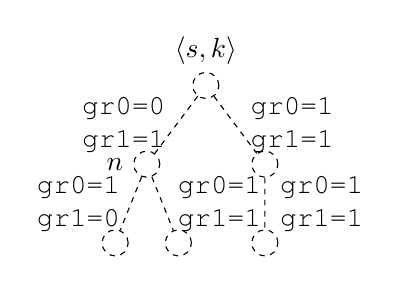
\begin{tikzpicture}[dash pattern = on 2pt off 2pt, level distance = 10mm]
            \node [circle,draw] (root){}
                child {node [circle,draw] {}
                    child {node [circle,draw,right=5pt] {}
                        edge from parent node [left=2pt,text width=1cm] {\texttt{gr0=1 gr1=0}}
                    }
                    child {node [circle,draw,left=5pt] {}
                        edge from parent node [right=2pt,text width=1cm] {\texttt{gr0=1 gr1=1}}
                    }
                    node [left=5pt] {$n$}
                    edge from parent node [left=2pt,text width=1cm] {\texttt{gr0=0 gr1=1}}
                }
                child {node [circle,draw] (n) {}
                    child {node [circle,draw] {}
                        edge from parent node [right=2pt,text width=1cm] {\texttt{gr0=1 gr1=1}}
                    }
                    edge from parent node [right=2pt,text width=1cm] {\texttt{gr0=1 gr1=1}}
                }
                node [above=4pt] {$\langle s, k \rangle$};
        \end{tikzpicture}
        \caption{A losing AGT $T$}
        \label{fig:interpolatetree}
    \end{subfigure}%
    \begin{subfigure}[t]{.32\textwidth}
        \centering
        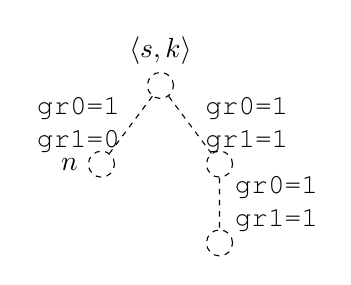
\begin{tikzpicture}[dash pattern = on 2pt off 2pt, level distance = 10mm]
            \node [circle,draw] (root){}
                child {node [circle,draw] {}
                    node [left=5pt] {$n$}
                    edge from parent node [left=2pt,text width=1cm] {\texttt{gr0=1 gr1=0}}
                }
                child {node [circle,draw] (n) {}
                    child {node [circle,draw] {}
                        edge from parent node [right=2pt,text width=1cm] {\texttt{gr0=1 gr1=1}}
                    }
                    edge from parent node [right=2pt=2pt=2pt=2pt,text width=1cm] {\texttt{gr0=1 gr1=1}}
                }
                node [above=4pt] {$\langle s, k \rangle$};
        \end{tikzpicture}
        \caption{Tree slice $T_1$}
        \label{fig:treef1}
    \end{subfigure}%
    \begin{subfigure}[t]{.32\textwidth}
        \centering
        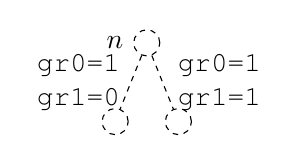
\begin{tikzpicture}[dash pattern = on 2pt off 2pt, level distance = 10mm]
            \node [circle,draw] {}
                child {node [circle,draw,right=5pt] {}
                    edge from parent node [left=2pt,text width=1cm] {\texttt{gr0=1 gr1=0}}
                }
                child {node [circle,draw,left=5pt] {}
                    edge from parent node [right=2pt,text width=1cm] {\texttt{gr0=1 gr1=1}}
                }
                node [left=5pt] {$n$};
        \end{tikzpicture}
        \caption{Tree slice $T_2$}
        \label{fig:treef2}
    \end{subfigure}
    \caption{Splitting of an abstract game tree by the learning procedure.}
    \label{fig:interpolanttrees}
\end{figure}

\begin{algorithm}[t]
    \begin{algorithmic}[1]
        \Require $s(X_T) \land $ \Call{treeFormula}{$k, T$} $\equiv \bot$
        \Require \emph{Must-invariant} holds
        \Ensure \emph{Must-invariant} holds
        \Ensure $s(X_T) \land B^M \not\equiv \bot$
        \Comment $s$ will be added to $B^M$
        \Function{learn}{$s, T$}
            \IIf{\Call{succ}{$T$} $= \emptyset$}
                \Return
            \EndIIf
            \State $n \gets $ non-leaf node with min height 
            \State $\langle T_1, T_2 \rangle \gets $ \Call{gtSplit}{$T, n$}
            \State $\mathcal{I} \gets $ \Call{interpolate}{$s(X_T) \land $ \Call{treeFormula}{$k, T_1$}, \Call{treeFormula}{$k, T_2$}}
            \State $B^M \gets B^M \lor \mathcal{I}$
            \State \Call{learn}{$s, T_1$}
        \EndFunction
        \algstore{learn}
    \end{algorithmic}
    
    \begin{algorithmic}[1]
        \algrestore{learn}
        \Require $s(X_T) \land $ \Call{\textoverline{treeFormula}}{$k, T$} $\equiv \bot$
        \Require \emph{May-invariant} holds
        \Ensure \emph{May-invariant} holds
        \Ensure $s(X_T) \land B^m[$\Call{height}{$k, T$}$] \equiv \bot$
        \Comment{$s$ will be removed from $B^m$}
        \Function{\textoverline{learn}}{$s, T$}
            \IIf{\Call{succ}{$T$} $= \emptyset$}
                \Return
            \EndIIf
            \State $n \gets $ non-leaf node with min height 
            \State $\langle T_1, T_2 \rangle \gets $ \Call{gtSplit}{$T, n$}
            \State $\mathcal{I} \gets $ \Call{interpolate}{$s(X_T) \land $ \Call{\textoverline{treeFormula}}{$k, T_1$}, \Call{\textoverline{treeFormula}}{$k, T_2$}}
            \For{$i = 1$ to \Call{height}{$k, n$}}
                \State $B^m[i] \gets B^m[i] \setminus \mathcal{I}$
            \EndFor
            \State \Call{\textoverline{learn}}{$s, T_1$}
        \EndFunction
    \end{algorithmic}
    \caption{Learning algorithms}
    \label{alg:learn}
\end{algorithm}

\begin{exmpInt}

    Consider node $n$ in Figure~\ref{fig:interpolatetree}. At this node there
    are two controller actions that prevent the environment from forcing the
    game into an error state in one game round. We want to use this tree to
    learn the states from which the controller can win playing one of these
    actions.

    One option is using a BDD solver, working backwards from the error set, to
    find all losing states. One iteration of this operation on our example
    would give the set: $\texttt{nrequests} = 3 \lor (\texttt{nrequests} = 2
    \land ( \texttt{resource0} = 0 \lor \texttt{resource1} = 0)) \lor
    (\texttt{nrequests} = 1 \land (\texttt{resource0} = 0 \land
    \texttt{resource1} = 0))$.  In the general case there is no compact
    representation of the losing set, so we try to avoid computing it by
    employing interpolation instead. The benefit of interpolation is
    that it allows approximating the losing states efficiently by obtaining 
    an interpolant from a SAT solver.
\end{exmpInt}


Given two formulas $F_1$ and $F_2$ such that $F_1 \land F_2$ is unsatisfiable,
it is possible to construct a Craig interpolant~\cite{craig1957} $\mathcal{I}$
such that $F_1 \to \mathcal{I}$, $F_2 \land \mathcal{I}$ is unsatisfiable, and
$\mathcal{I}$ refers only to the intersection of variables in $F_1$ and $F_2$.
An interpolant can be constructed efficiently from a resolution proof of the
unsatisfiability of $F_1 \land F_2$~\cite{pudlak1997}.

We choose a non-leaf node $n$ of $T$ with maximal depth, i.e., a node whose
children are leafs (Algorithm~\ref{alg:learn}, line~3). We then split the tree
at $n$ such that both slices $T_1$ and $T_2$ contain a copy of $n$ (line~4).
Figure~\ref{fig:treef1} shows $T_1$, which contains all of $T$ except $n$'s
children, and $T_2$ (Figure~\ref{fig:treef2}), which contains only $n$ and its
children.  There is no candidate strategy for $T$ so $s \land
\textsc{\textoverline{treeFormula}}(k, T)$ is unsatisfiable.  By construction,
$\textsc{\textoverline{treeFormula}}(k, T) \equiv
\textsc{\textoverline{treeFormula}}(k, T_1) \land
\textsc{\textoverline{treeFormula}}(k, T_2)$ and hence $s \land
\textsc{\textoverline{treeFormula}}(k, T_1) \land
\textsc{\textoverline{treeFormula}}(k, T_2)$ is also unsatisfiable.

%%%This enables the construction of an interpolant that captures losing states at
%%%node $n$.

We construct an interpolant with $F_1 = s(X_T) \land \textsc{treeFormula}(k,
T_1)$ and $F_2 = \textsc{treeFormula}(k, T_2)$ (line~5). The only variables
shared between $F_1$ and $F_2$ are the state variable copies belonging to node
$n$. By the properties of the interpolant, $F_2 \land \mathcal{I}$ is
unsatisfiable, therefore all states in $\mathcal{I}$ are losing against
abstract game tree $T_2$ in Figure~\ref{fig:treef2}.  We also know that $F_1
\to \mathcal{I}$, thus $\mathcal{I}$ contains all states reachable at $n$ by
following $T_1$ and avoiding error states. 

\begin {exmp}

    At node $n$, the interpolant $\texttt{nrequests} = 1 \land
    \texttt{resource1} = 1$ captures the information we need. Any action by the
    environment followed by one of the controller actions at $n$ will be
    winning for the controller.

\end{exmp}

We have discovered a set $\mathcal{I}$ of states losing for the environment.
Environment-losing states are only losing for a particular bound: given that
there does not exist an environment strategy that forces the game into an error
state in $k$ rounds or less; there may still exist a longer environment-winning
strategy.  We therefore record learned environment-losing states along with
associated bounds.  To this end, we maintain a conceptually infinite array of
sets $B^m[k]$ that are may-losing for the controller, indexed by bound $k$.
$B^m[k]$ are initialised to $E$ for all $k$.  Whenever an environment-losing
set $\mathcal{I}$ is discovered for a node $n$ with bound $\textsc{height}(k,
n)$ in line~13 of Algorithm~\ref{alg:learn}, this set is subtracted from
$B^m[i]$, for all $i$ less than or equal to the bound (lines~14--16).

The \textsc{\textoverline{treeFormula}} function is modified for the unbounded
solver (Algorithm~\ref{alg:unboundedTreeFormula}) to constrain the environment
to the appropriate $B^m$. This enables further interpolants to be constructed
by the learning procedure recursively splitting more nodes from $T_1$
(Algorithm~\ref{alg:learn}, line~7) since the states that are losing to $T_2$
are no longer contained in $B^m$.

\begin{algorithm}[t] \caption{Amended tree formulas for Controller and
    Environment} \label{alg:unboundedTreeFormula} \begin{algorithmic}[1]
        \Function{treeFormula}{$k, T$} \If{$\Call{height}{k, T} = 0$} \State
        \Return{ $\lnot \Call{$B^M$}{X_{T}}$ } \Else \State \Return{$\lnot
            \Call{$B^M$}{X_{T}} \land$ \\ $$\bigwedge_{\langle e, n \rangle \in
            \Call{succ}{T}}(\Call{$\delta$}{X_T, U_e, C_n, X_n} \land U_e =
            \Call{action}{e} \land \Call{treeFormula}{k, n})$$ } \EndIf
        \EndFunction \algstore{tf1} \end{algorithmic}

    \begin{algorithmic}[1]
        \algrestore{tf1}
        \Function{\textoverline{treeFormula}}{$k, T$}
        \If{$\Call{height}{k, T} = 0$}
        \State \Return{\Call{E}{$X_T$}}
        \Else
        \State \Return{ \Call{$B^m[\Call{height}{k, T}]$}{$X_{T}$} $\land$ \\
            $$\bigg( \Call{E}{X_T} \lor \bigvee_{\langle e, n \rangle \in \Call{succ}{T}}(\Call{$\delta$}{X_T, U_n, C_e, X_n} \land C_e = \Call{action}{e} \land \Call{\textoverline{treeFormula}}{k, n})\bigg)$$ }
        \EndIf
        \EndFunction
    \end{algorithmic}
\end{algorithm}

Learning of states losing from the controller is similar (\textsc{learn} in
Algorithm~\ref{alg:learn}). The main difference is that environment-losing
states are losing for all bounds. Therefore we record these states in a single
set $B^M$ of must-losing states (Algorithm~\ref{alg:learn}, line~6).  This set
is initialised to the error set $E$ and grows as new losing states are
discovered.  The modified \textsc{\textoverline{treeFormula}} function
(Algorithm~\ref{alg:unboundedTreeFormula}) blocks must-losing states, which
also allows for recursive learning over the entire tree.

\subsection{Main synthesis loop}

Figure~\ref{alg:unbounded} shows the main loop of the unbounded synthesis algorithm.
The algorithm invokes the modified bounded synthesis procedure with increasing bound $k$
until the initial state is in $B^M$ (environment wins) or $B^m$ reaches a fixed point 
(controller wins). We prove correctness in the next section.

\begin{algorithm}[h]
    \begin{algorithmic}[1]
        \Function{solveUnbounded}{$T$}
            \State $B^M \gets E$
            \State $B^m[0] \gets E$
            \For{$k = 1 \dots$}
                \IIf{\Call{SAT}{$I \land B^M$}}
                    \Return \texttt{unrealisable} \Comment{Losing in the initial state}
                \EndIIf
                \IIf{$\exists i < k . \  B^m[i] \equiv B^m[i+1]$} \Comment{Reached fixed point}
                    \State \hspace{\algorithmicindent} \Return \texttt{realisable} 
                \EndIIf
                \State $B^m[k] \gets E$
                \State \Call{checkBound}{$k$}
            \EndFor
        \EndFunction
        \algstore{u1}
    \end{algorithmic}

    \begin{algorithmic}
        \algrestore{u1}
        \Require \emph{May} and \emph{must} invariants hold
        \Ensure \emph{May} and \emph{must} invariants hold
        \Ensure $I \not\in B^m[k]$ if there exists a winning controller strategy with bound $k$
        \Ensure $I \in B^M$ if there exists a winning environment strategy with bound $k$
%%%        $\exists u_{k..1} \forall c_{k..1} \  s(x_k) \land (E_k \lor (\delta(x_k, u_k, c_k) \land E(x_{k-1}) \lor ... \land E(x_1) \lor (\delta(x_1, u_1, c_1) \land E(x_0))...)$
%%%            $\forall u_{k..1} \exists c_{k..1} \  s(x_k) \land \lnot E_k \land \delta(x_k, u_k, c_k) \land \lnot E(x_{k-1}) \land ... \land \delta(x_1, u_1, c_1) \land \lnot E(x_0)$
        \Function{checkBound}{$k$}
            \State \Return \Call{solveAbstract}{$\texttt{env}, I, k, \emptyset$}
        \EndFunction
    \end{algorithmic}
    \caption{Unbounded Synthesis}
    \label{alg:unbounded}
\end{algorithm}



\subsection{Correctness}


We define two global invariants of the algorithm.  The \emph{may-invariant}
states that sets $B^m[i]$ grow monotonically with $i$ and that each $B^m[i+1]$
overapproximates the states from which the environment can force the game into
$B^m[i]$. We call this operation $Upre$, the uncontrollable predecessor. So the
\emph{may-invariant} is: $$\forall i<k.~B^m[i] \subseteq B^m[i+1], Upre(B^m[i])
\subseteq B^m[i+1].$$

The \emph{must-invariant} guarantees that the must-losing set $B^M$ is an
underapproximation of the actual losing set $B$: $$B^M \subseteq B.$$

Correctness of $\textsc{solveUnbounded}$ follows from these invariants. The
must-invariant guarantees that the environment can force the game into an error
state from $B^M$, therefore checking whether the initial state is in $B^M$ (as
in line~5) is sufficient to return \texttt{unrealisable}. The may-invariant
tells us that if $B^m[i] \equiv B^m[i+1]$ (line~6) then $Upre(B^m[i]) \subseteq
B^m[i]$, i.e. $B^m[i]$ overapproximates the winning states for the environment.
We know that $I \not\in B^m[k]$ due to the post-condition of
\textsc{checkBound}, and since the may-invariant tells us that $B^m$ is
monotonic then $I$ must not be in $B^m[i]$. If $I \not\in B^m[i]$ then $I$ is
not in the winning states for the environment and the controller can always win
from $I$. 

Both invariants trivially hold after $B^m$ and $B^M$ have been initialised in
the beginning of the algorithm. The sets $B^m$ and $B^M$ are only modified by
the functions \textsc{learn} and \textoverline{\textsc{learn}}.  Below we prove
that \textoverline{\textsc{learn}} maintains the invariants.  The proof of
\textsc{learn} is similar.

\subsection{Proof of \textoverline{\textsc{learn}}}

We prove that postconditions of \textsc{\textoverline{learn}} are satisfied
assuming that its preconditions hold.

Line~(11--12) splits the tree $T$ into $T_1$ and $T_2$, such that $T_2$ has depth
1.  Consider formulas $F_1=s(X_T) \land
\textsc{\textoverline{treeFormula}}(k, T_1)$ and $F_2 =
\textsc{\textoverline{treeFormula}}(k, T_2)$.  These formulas only share variables
$X_n$.  Their conjunction $F_1 \land F_2$ is unsatisfiable, as by construction
any solution of $F_1 \land F_2$ also satisfies $s(X_T) \land
\textsc{\textoverline{treeFormula}}(k, T)$, which is unsatisfiable (precondition (b)).  Hence the
interpolation operation is defined for $F_1$ and $F_2$.  

Intuitively, the interpolant computed in line~(13) overapproximates the set of
states reachable from $s$ by following the tree from the root node to $n$,
and underapproximates the set of states from which the environment loses
against tree $T_2$.  

Formally, $\II$ has the property $\II \land F_2 \equiv \bot$.  Since $T_2$ is
of depth 1, this means that the environment cannot force the game into
$B^m[\textsc{height}(k, n)-1]$ playing against the counterexample moves in $T_2$.
Hence, $\II \cap Upre(B^m[\textsc{height}(k, n)-1]) = \emptyset$.  Furthermore,
since the may-invariant holds, $\II \cap Upre(B^m[i]) =
\emptyset$, for all $i < \textsc{height}(k, n)$.  Hence, removing $\II$ from all
$B^m[i], i\leq \textsc{height}(k, n)$ in line~(15) preserves the may-invariant,
thus satisfying the first post-condition.

Furthermore, the interpolant satisfies $F_1 \rightarrow \II$, i.e., any
assignment to $X_n$ that satisfies $s(X_T) \land
\textsc{\textoverline{treeFormula}}(k, T_1)$ also satisfies $\II$.  Hence,
removing $\II$ from $B^m[\textsc{height}(k, n)]$ makes $s(X_T) \land
\textsc{\textoverline{treeFormula}}(k, T_1)$ unsatisfiable, and hence all
preconditions of the recursive invocation of \textsc{\textoverline{learn}} in
line~(17) are satisfied.  

At the second last recursive call to \textsc{\textoverline{learn}}, tree $T_1$
is empty, $n$ is the root node, $\textsc{\textoverline{treeFormula}}(k, T_1)
\equiv B^m[\textsc{height}(k, T_1)](X^T)$; hence $s(X_T) \land
\textsc{\textoverline{treeFormula}}(k, T_1) \equiv s(X_T) \land
B^m[\textsc{height}(k, T_1)](X^T) \equiv \bot$.  Thus the second postcondition of
\textsc{\textoverline{learn}} holds.

The proof of \textsc{learn} is similar to the above proof of \textsc{learn}. An
interpolant constructed from $F_1=s(X_T) \land \textsc{treeFormula}(k, T_1)$
and $F_2 = \textsc{treeFormula}(k, T_2)$ has the property $\II \land F_2 \equiv
\bot$ and the precondition ensures that the controller is unable to force the
game into $B^M$ playing against the counterexample moves in $T_2$. Thus adding
$\II$ to $B^M$ maintains the must-invariant satisfying the first postcondition.

Likewise, in the second last recursive call of \textsc{learn} with the empty
tree $T_1$ and root node $n$: $\textsc{treeFormula}(k, T_1) \equiv \lnot
B^M(X_T)$.  Hence $s(X_T) \land \textsc{treeFormula}(k, T_1) \equiv
s(X_T) \land \lnot B^M(X_T) \equiv \bot$. Therefore $s(X_T) \land
B^M(X_T) \not\equiv \bot$, the second postcondition, is true.

\subsection{Proof of Termination}

We must prove that $\textsc{checkBound}$ terminates and that upon termination
its postcondition holds, i.e., state $I$ is removed from $B^m[\kappa]$ if there
is a winning controller strategy on the bounded safety game of maximum bound
$\kappa$ or it is added to $B^M$ otherwise. Termination follows from
completeness of counterexample guided search, which terminates after
enumerating all possible opponent moves in the worst case.

Assume that there is a winning strategy for the controller at bound $\kappa$.
This means that at some point the algorithm discovers a counterexample tree of
bound $\kappa$ for which the environment cannot force into $E$. The algorithm
then invokes the \textsc{\textoverline{learn}} method, which removes $I$ from
$B^m[\kappa]$.  Alternatively, if there is a winning strategy for the
environment at bound $\kappa$ then a counterexample losing for the controller
will be found.  Subsequently \textsc{learn} will be called and $I$ added to
$B^M$.

\subsection{Optimisation: Generalising the initial state}

This optimisation allows us to learn may and must losing states faster.
Starting with a larger set of initial states we increase the reachable set and
hence increase the number of states learned by interpolation. This optimisation
requires a modification to $\textsc{solveAbstract}$ to handle sets of states,
which is not shown.

The optimisation is relatively simple and is inspired by a common greedy
heuristic for minimising $\texttt{unsat}$ cores. Initial state $I$ assigns a value to
each variable in $X$. If the environment loses $\langle I, k
\rangle$ then we attempt to solve for a generalised version of $I$ by removing
one variable assignment at a time. If the environment loses from the larger set of
states then we continue generalising. In this way we learn more
states by increasing the reachable set. In our benchmarks we have observed that
this optimisation is beneficial on the first few iterations of
\textsc{checkBound}.

\begin{algorithm}
    \begin{algorithmic}
        \Function{checkBound}{$k$}
            \State $r \gets $ \Call{solveAbstract}{$\texttt{env}, I, k, \emptyset$}
            \IIf{$r \neq \emptyset$} \Return $r$ \EndIIf
            \State $s' \gets I$
            \For{$x \in X$}
            \State $r \gets$ \Call{solveAbstract}{$\texttt{env}, s' \setminus \{x\}, k, \emptyset$} 
                \IIf{$r = \texttt{NULL}$} $s' \gets s' \setminus \{x\}$ \EndIIf \Comment{Removes the assignment to $x$ from $s'$}
            \EndFor
            \State \Return $\texttt{NULL}$
        \EndFunction
    \end{algorithmic}
    \caption{Generalise $I$ optimisation}
    \label{alg:opt1}
\end{algorithm}

\begin{algorithm}
    \begin{algorithmic}[1]
        \Function{solveAbstract}{$p, s, k, T$}
        \State $cand \gets $ \Call{findCandidate}{$p, s, k, T$} \Comment{Look for a candidate}
        \IIf{$k = 1$} \Return $cand$ \EndIIf \Comment{Reached the bound}
        \State $T' \gets T$
        \Loop
            \IIf{$cand = \texttt{NULL}$} \Return $\texttt{NULL}$ \EndIIf \Comment{No candidate: return with no solution}
            \State $\langle cex, l, u \rangle \gets $ \Call{verify}{$p, s, k, T, cand$} \Comment{Verify candidate}
            \IIf{$cex = \False$} \Return $cand$ \EndIIf \Comment{No counterexample: return candidate}
            \State $T' \gets $ \Call{append}{$T', l, u$} \Comment{Refine $T'$ with counterexample}
            \State $cand \gets $ \Call{solveAbstract}{$p, s, k, T'$} \Comment{Solve refined game tree}
        \EndLoop
        \EndFunction
        \algstore{b1}
    \end{algorithmic}

    \begin{algorithmic}
        \algrestore{b1}
        \Function{findCandidate}{$p, s, k, T$}
        \State $\hat{T} \gets $ \Call{extend}{$T$} \Comment{Extend the tree with unfixed actions}
            \State $f \gets $ \IfElse{$p = \texttt{cont}$}{\Call{treeFormula}{$k, \hat{T}$}}{\Call{\textoverline{treeFormula}}{$k, \hat{T}$}} \EndIfElse
            \State $sol \gets $ \Call{SAT}{$s(X_{\hat{T}}) \land f$}
            \If{$sol = \texttt{unsat}$} 
                \If{\texttt{unbounded}} \Comment{Active only in the unbounded solver}
                    %\State $\sigma \gets $ \Call{generalise}{$s$} \Comment{Expand $s$ to a set of states}
                    \State \IfElse{$p = \texttt{cont}$}{\Call{learn}{$s, \hat{T}$}}{\Call{\textoverline{learn}}{$s, \hat{T}$}} \EndIfElse
                \EndIf
                \State \Return $\texttt{NULL}$ \Comment{No candidate exists}
            \Else
                \State \Return $\{ \langle n, c \rangle | n \in $ \Call{nodes}{$T$} $, c = \Call{sol}{n} \}$ \Comment{Fix candidate moves in $T$}
            \EndIf
        \EndFunction
        \algstore{b2}
    \end{algorithmic}

    \begin{algorithmic}
        \algrestore{b2}
        \Function{verify}{$p, s, k, T, cand$}
            \For{$l \in leaves(gt)$}
            \State $\langle k', s'\rangle \gets $ \Call{outcome}{$s, k, cand, l$} \Comment{Get bound and state at leaf}
            \State $T' \gets$ \IfElse{$p = \textsc{cont}$}{$\emptyset$}{$\{ cand(l) \}$ } \EndIfElse
                \State $a \gets $ \Call{solveAbstract}{\Call{opponent}{$p$}, $s'$, $k'$, $T'$} \Comment{Solve for the opponent}
                \IIf{$a \neq \texttt{NULL}$} \Return $\langle \True, l, a \rangle$ \EndIIf \Comment{Return counterexample}
            \EndFor
            \State \Return $\langle \False, \emptyset, \emptyset \rangle$
        \EndFunction
    \end{algorithmic}

    \caption{Bounded synthesis}
    \label{alg:bounded}
\end{algorithm}


\chapter{Evaluation}

\chapter{Conclusion}

\bibliographystyle{thesisnat}
\bibliography{main}

\end{document}
